\chapter{Présententation de l'entreprise}
\section{Naissance et évolution}
\paragraph*{}
La société Luxembourg Online est une société anonyme (SA) fondée en 1995 et elle est implentée uniquement sur le territoire luxembourgeois. La société est l'un des principaux opérateurs luxembourgeois de télécommunications et est spécialisée dans la fourniture d'accès internet, la téléphonie fixe, mobile, la télévision, le développement de réseaux et d'applications informatiques. Depuis sa création en 1995 la société a fait de manière récurrente à intervalle de plus ou moins 2 ans des lancements majeures de services.  En 1997, elle lance sa plateforme de commerce électronique, deux ans plus tard en 1999 elle lance un accès internet gratuit à une échelle nationale. En 2001 il y a eu le lancement des forfaits internet sous forme de packages, en 2003, elle lance l'accès à internet par le câble de télévision et de l'accès internet haut-débit. En 2004 elle lance le service de préselection téléphonique Luxembourg Online pour téléphoner moins cher. En 2005, elle lance le service de téléphonie via internet et deux ans plus tard le service de téléphonie mobile. En 2011, elle lance un service de TV qui est une solution de télévision par \gls{IP} et deux ans plus tard elle lance le dégroupage en fibre optique. Enfin en 2016 elle lance le service de visiophonie.

\begin{figure}[H]
	\centering
	
\includegraphics[scale=1]{assets/images/Logo-LOL.png}
	\caption{Logo de la société Luxembourg Online}
	\label{fig.1}
\end{figure} 

\section{Effectif, organisation et services de la société}
La société Luxembourg Online dispose d'un effectif de plus de 100 collaborateurs, répartis sur 3 sites dans le pays. Le siège de la société est situé dans la ville de Luxembourg le lieu de mon stage. Dans ces bureaux sont installés : le service informatique dans lequel j'ai travaillé, le service administratif et le service comptabilité. Les deux autres sites sont situés respectivement dans la ville de Luxembourg qui sert de boutique oú est intallé le service client et les vendeurs et dans la ville de Bertrange qui est un lieu de stockage de tous les matériels de télécommunications (équipements fibre optique, box internet, câble de raccordements, et les décodeurs TV).
\paragraph*{}
La société dispose de son propre réseau internet sur le territoire Luxembourgeois et qui couvre presque la totalité du pays. Elle dispose aussi de son propre réseau de téléphonie fixe par \gls{IP} et de télévision par \gls{IP}. Cette autonomie permet à la société  d'être totalement libre sur le développement, la commercialisation et le suivi de l'ensemble de ses services et produits. La société propose à ses clients plusieurs offres internet qui va de la connexion bas débit \gls{DSL} à une connexion très haut-débit par fibre optique. Les-dits clients peuvent de manière optionnelle souscrire au service de télévision, de téléphonie ou encore de stockage cloud.

\begin{figure}[H]
	\centering
	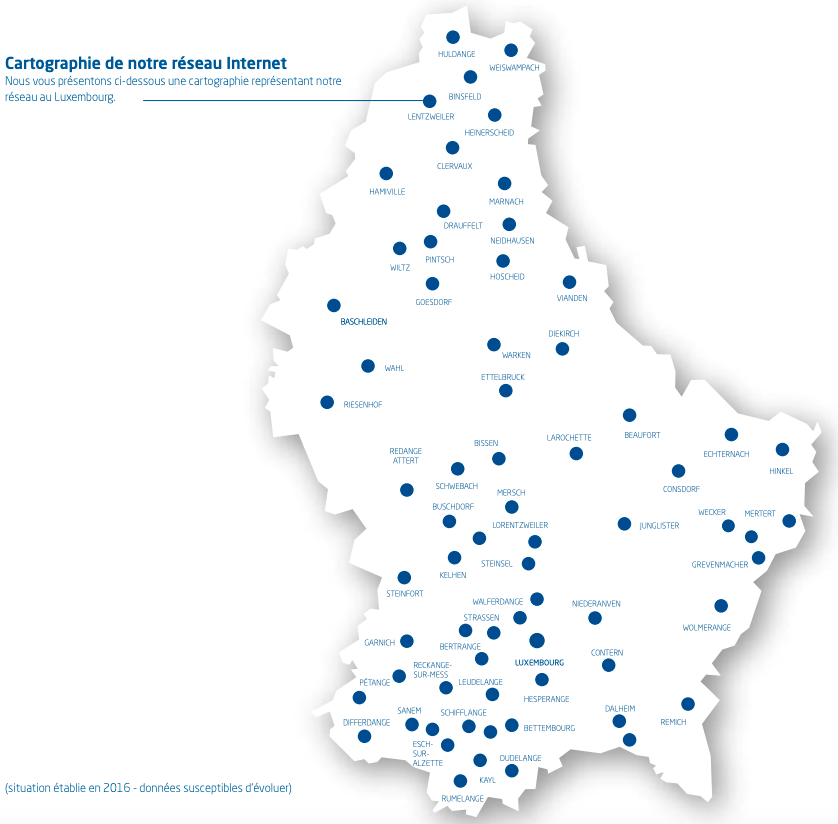
\includegraphics[scale=0.3]{assets/images/cartographie}
	\caption{Cartographie du réseau de fibre optique couverte par la société}
	\label{fig.2}
\end{figure}

\paragraph*{}

Outre son activité de \gls{FAI}, Luxembourg Online est un opérateur de téléphonie mobile et une société de service informatique qui développe des solutions informatiques pour le grand public et pour toute sorte d'entreprise.

\section{Ouverture sur mon travail au cours du stage}
\paragraph*{}
Le service qui m'a accueilli pendant mon stage est le service informatique. J'ai travaillé dans un premier temps seul sur un premier projet et je faisais des rapports à M. \textbf{Paul RETTER} qui est mon tuteur en entreprise et j'ai ensuite travaillé sur un deuxième projet sous la direction toujours de mon tuteur  mais cette fois-ci en collaboration avec d'autres ingénieurs de la société.